\documentclass[a4, 12pt,titlepage]{scrartcl}

\usepackage[margin=1cm]{geometry}
\usepackage{nopageno}
\usepackage{amssymb}
\usepackage{amsmath}
\usepackage{graphicx}
\graphicspath{ {Attached graph} }

\title{Statistics}
\subtitle{Introduction to Data Science - 2020 Semester A Final Project}
\author{Ori Darshan: 212458244}
\date{}

\begin{document}

\maketitle

\bigskip
\section{Probability and Bayes Theorem}
\subsection{Question 1}
\subsubsection{Section a:}
\textbf{\underline{Question:}}\\
Around 1/125 of all births are nonidentical twins, and 1/300 are identical twins. Elvis had a twin brother who died in birth. What is the probability that Elvis had an identical twin?\\
(you can assume that the probability for boys/girls is 1/2)\\\smallskip\\
\textbf{\underline{Answer:}}\\
We search for the probability of Elvis to have an identical twin.
The general probability is 1/300 (given). How the information we have affects that number?\\
We know that Elvis had a twin, from all possibilities, 1/300 is the chance for an identical and 1/125 are the chances for a nonidentical twins.\\
combining these two option we get\[
\frac{1}{300}+\frac{1}{125}=\frac{17}{1500}
\]

We won't actually use this number, since we know that Elvis had a twin we will look only on the `twin related' statistics.\\
From all possibilities for twins, what is the probability for an identical twins?\begin{align*}
\intertext{identical:}
\frac{1}{300}/\frac{17}{1500}&=\frac{5}{17}\\
\intertext{nonidentical:}
\frac{1}{125}/\frac{17}{1500}&=\frac{12}{17}\\
\end{align*}

We know that the twin was a boy, all of the identical twins are the same gender while only 1/2 of the nonidentical twins will have the same gender (given).\\
Elvis can be part of the 1/300 births of identical twins or part of the $(1/125)/2=1/250$ births of nonidentical, same-gender births.\\
The probability for a same gender twin from all possible twins is:
\begin{align*}
P(\textrm{same gender twins})&=\frac{5}{17}+0.5\cdot \frac{12}{17}\\\smallskip\\
&=\frac{11}{17}
\end{align*}
We will use Bayes theorem to calculate the probability for an identical twin given there was a twin from the same gender, as a base we will use the probabilities shown above for identical twins given there was a twin.\[
P(\textrm{identical $|$ same gender})=\frac{P(\textrm{same gender $|$ identical})\cdot P(\textrm{identical})}{P(\textrm{same gender})}
\]Inserting previous calculations:
\begin{align*}
P(\textrm{identical $|$ same gender})&=\frac{1\cdot \frac{5}{17}}{\frac{11}{17}}=\frac{5}{11}
\end{align*}
The probability Elvis's twin was an identical twin is:
\[
\boxed{P=\frac{5}{11}}
\]
\newpage
\subsubsection{Section b}
\textbf{\underline{Question:}}\\
There are two cookie bowls, in Bowl 1 there are 10 almond cookies and 30 chocolate cookies. in Bowl 2 there are 20 almond cookies and 20 chocolate cookies.\\
Eric chose a random bowl and took 1 random cookie from it. the cookie was a chocolate cookie.\\
What is the probability that Eric chose Bowl 1?\\
\textbf{\underline{Answer:}}\\
The probability to pick Bowl 1 is 1/2 (Bowl 1 or Bowl 2),
The probability to pick a chocolate cookie is 50/80=5/8.\\
Given the cookie was chocolate cookie, the probability for choosing Bowl 1 changes according to Bayes theorem:\\
\[
P(\textrm{bowl 1 $|$ chocolate cookie})=\frac{P(\textrm{chocolate cookie $|$ Bowl 1})\cdot P(\textrm{Bowl 1})}{P(\textrm{chocolate cookie})}
\]
Inserting known probabilities:
\[
P(\textrm{bowl 1 $|$ chocolate cookie})=\frac{\frac{3}{4}\cdot \frac{1}{2}}{\frac{5}{8}}=\frac{3}{5}
\]
The probability Eric chose Bowl 1 is:
\[
\boxed{P=\frac{3}{5}}
\]
\newpage

\subsection{Question 2}
\textbf{\underline{Question:}}\\
In 1995, M\&M company added the blue color. before this year, the color distribution was:\[
\textrm{30\% Brown, 20\% Yellow, 20\% Red, 10\% Green, 10\% Orange, 10\% Tan}
\]
Since 1995, the distribution looks like that:\[
\textrm{24\% Blue, 20\% Green, 16\% Orange, 14\% Yellow, 13\% Red, 13\% Brown}
\]
Your friend have 2 M\&M bags, one from 1994 and one from 1996 and he is not willing to expose which one belongs to which year. But he gives you one candy from each bag. one candy is yellow and the other one is green.\\
What is the probability that the yellow candy came from the bag of 1994?\\

\textbf{\underline{Answer:}}\\
At first glance on the distributions, we can see that the green candy is more likely to come from the 1996's bag while the yellow candy is more likely to come from the 1994's bag. Let's calculate that.\\

Assuming Eric chose the candies at random (otherwise Eric decided what option is true), we need to calculate these parameters in order to use Bayes theorem:
\begin{center}
\quad P(1 yellow, 1 green $|$ yellow from 1994),\quad P(yellow from 1994), \quad P(1 green, 1 yellow)
\end{center}\smallskip
\begin{align*}
&\textrm{P(1 yellow, 1 green $|$ yellow from 1994)}=\textrm{P(green in 1996)}=0.2\\
&\textrm{P(yellow from 1994)}=0.2\\
&\textrm{P(1 green, 1 yellow) = P(green 1994, yellow 1996) + P(green 1996, yellow 1994)}\\
&\qquad=0.1\cdot 0.14+0.2\cdot 0.2=0.054\\
\end{align*}Using Bayes theorem, we get:\[
P(\textrm{yellow from 1994 $|$ 1 green, 1 yellow})=\frac{P(\textrm{1 green, 1 yellow $|$ yellow from 1994})\cdot P(\textrm{yellow from 1994})}{P(\textrm{1 green, 1 yellow})}
\]
With the statistics discovered earlier:\[
P(\textrm{yellow from 1994 $|$ 1 green, 1 yellow})=\frac{0.2\cdot 0.2}{0.054}=\frac{20}{27}
\]
This result align with our assumption.\\\smallskip\\
The probability the yellow candy is from the 1994's bag is:
\[
\boxed{P=\frac{20}{27}}
\]
\newpage


\subsection{Question 3}
\textbf{\underline{Question:}}\\
You went to the doctor due to an ingrown toenail. The doctor chose you at random to make a Swine influenza test. It is known that 1 out of 10,000 are infected by Swine influenza. The test is 99\% accurate in the sense that the probability for a false positive is 1\%. which means that the probability a healthy man was diagnosed as ill is 1\%. The probability for false negative (ill man as healthy) is 0\%.\\
You was found positive to Swine influenza.\\

\noindent
\underline{a:} What is the probability you have Swine influenza?\\
\underline{b:} Let's say you returned from Thailand lately, and you know that 1 out of 200 people who returned from Thailand lately return with Swine influenza.\\
Given the same situation like section a. What is the (updated) probability you have Swine influenza? \\
\smallskip\\

\noindent
\textbf{\underline{Answer a:}}\\
To use Bayes theorem, we need to find what is the probability you will get a positive test. \[
\textrm{P(positive)=P(ill)+P(healthy but positive)}=\frac{1}{10000}+\frac{9999}{10000}\cdot \frac{1}{100}=\frac{10099}{1000000}=0.010099
\]
Now using Bayes theorem we get:\[
P(\textrm{ill $|$ positive})=\frac{P(\textrm{positive $|$ ill})\cdot P(\textrm{ill})}{P(\textrm{positive})}
\]
\[
P(\textrm{ill $|$ positive})=\frac{1\cdot 0.0001}{0.010099}=\frac{100}{10099}
\]
Given a positive test, the probability you are ill is:\[
\boxed{P=\frac{100}{10099}}
\]
\smallskip\\
\textbf{\underline{Answer b:}}\\
We will update the parameters for P(ill) and P(positive) according to the new information.\\
The probability for getting a positive result will be:\[
\textrm{P(positive)=P(ill)+P(healthy but positive)}=\frac{1}{200}+\frac{199}{200}\cdot \frac{1}{100}=\frac{100}{20000}+\frac{199}{20000}=\frac{299}{20000}
\]
Now back to Bayes:\[
P(\textrm{ill $|$ positive})=\frac{P(\textrm{positive $|$ ill})\cdot P(\textrm{ill})}{P(\textrm{positive})}
\]
\[
P(\textrm{ill $|$ positive})=\frac{1\cdot \frac{1}{200}}{\frac{299}{20000}}=\frac{100}{299}
\]Given positive test and that you came back from Thailand, the probability you are ill is:\[
\boxed{P=\frac{100}{299}}
\]
\newpage

\section{Random Variables}
\subsection{Question 1}
\textbf{\underline{Question}}\\
Roi is playing a dice game with Yael.\\
Roi will roll 2 six-sided dice, and if the sum of the dice is divisible by 3, he will win 6\$.
If the sum is not divisible by 3, he will lose 3\$.\\
What is Roi's expected value of playing this game?\\
\smallskip\\
\textbf{\underline{Answer }}\\
For Roi to get 3\$ the dice sum must be divisible by 3. Between 1 and 12 the numbers divisible by 3 are 3,6,9,12. In any other option Roi will lose 3\$.\\
\smallskip\\
The probability for winning is:
\begin{align*}
&P(3)+P(6)+P(9)+P(12)\\
&\frac{2}{36}+\frac{5}{36}+\frac{4}{36}+\frac{1}{36}=\frac{12}{36}=\frac{1}{3}
\end{align*}
The probability for losing is $\frac{24}{36}=\frac{2}{3}$\\
Calculating the expected value, we get:\[
3\cdot \frac{1}{3}+(-3)\cdot \frac{2}{3}=-1
\]
\begin{center}
\boxed{\textrm{Roi's expected value of playing the game is -1\$}}
\end{center}
\subsection{Question 2}
\textbf{\underline{Question}}\\
Sharon has challenged Alex to a round of Marker Mixup.
Marker Mixup is a game where there is a bag of 5 red markers numbered 1 through 5, and another bag with 5 green markers numbered 6 through 10.\\
Alex will grab 1 marker from each bag, and if the 2 markers add up to more than 12, he will win 5\$, If the sum is exactly 12, he will break even, and If the sum is less than 12, he will
lose 6\$.\\
What is Alex's expected value of playing Marker Mixup?\\
\smallskip\\
\textbf{\underline{Answer}}\\
The possible outcomes are the following:\[
\begin{array}{c|ccccc}
& 1 & 2 & 3 & 4 & 5\\
\hline
6 & 7 & 8 & 9 & 10 & 11\\
7 & 8 & 9 & 10 & 11 & 12\\
8 & 9 & 10 & 11 & 12 & 13\\
9 & 10 & 11 & 12 & 13 & 14\\
10 & 11 & 12 & 13 & 14 & 15\\
\end{array}
\]
Above 12: $\frac{6}{25}$\quad exactly 12: $\frac{4}{25}$\quad below 12: $\frac{15}{25}$\\
The expected value will be:\[
5\cdot \frac{6}{25}+0\cdot \frac{4}{25}+ (-6)\cdot \frac{15}{25}=-2.4
\]
\begin{center}
\boxed{\textrm{Alex's expected value of playing Marker Mixup is -2.4\$}}
\end{center}
\newpage

\subsection{Question 3}
\textbf{\underline{Question}}\\
A division of a company has 200 employees, 40\% percent of which are male. Each month, the company randomly selects 8 of its employees to have lunch with the CEO.\\
What are the mean and standard deviation of the number of males selected each
month?\\
\smallskip\\
\textbf{\underline{Answer}}\\
The mean is the expected value, so:\[
8\textrm{\tiny (employees per month)}\cdot 0.4\textrm{\tiny (the probability they are male)}=\boxed{3.2}\]\\
The standard deviation will be calculated by the square root of the variance \\
First we find the variance, the variance is the squared deviation multiplied by the probability.\\
For each instance, the probability will be a ``branch'' in the probability tree for the problem multiplied by the time this probability occurs (binomial coefficient).\\
The reason is that if you look at the tree, the same outcomes will have the same numerators and the same denominators overall.
We will calculate the probability for each instance:\\
\begin{align*}
&P(\textrm{0 males}) =\binom{8}{0}\cdot \frac{120\cdot119\cdot118\cdot117\cdot116\cdot115\cdot114\cdot113}{200\cdot199\cdot198\cdot197\cdot196\cdot195\cdot194\cdot193} =0.0153
\\
&P(\textrm{1 male})\ =\binom{8}{1}\cdot \frac{120\cdot119\cdot118\cdot117\cdot116\cdot115\cdot114\cdot80}{200\cdot199\cdot198\cdot197\cdot196\cdot195\cdot194\cdot193}=0.0864
\\
&P(\textrm{2 males})=\binom{8}{2}\cdot \frac{120\cdot119\cdot118\cdot117\cdot116\cdot115\cdot80\cdot79}{200\cdot199\cdot198\cdot197\cdot196\cdot195\cdot194\cdot193}=0.2095
\\
&P(\textrm{3 males})=\binom{8}{3}\cdot \frac{120\cdot119\cdot118\cdot117\cdot116\cdot80\cdot79\cdot78}{200\cdot199\cdot198\cdot197\cdot196\cdot195\cdot194\cdot193}=0.2842
\\
&P(\textrm{4 males})=\binom{8}{4}\cdot \frac{120\cdot119\cdot118\cdot117\cdot80\cdot79\cdot78\cdot77}{200\cdot199\cdot198\cdot197\cdot196\cdot195\cdot194\cdot193}=0.2358
\\
&P(\textrm{5 males})=\binom{8}{5}\cdot \frac{120\cdot119\cdot118\cdot80\cdot79\cdot78\cdot77\cdot76}{200\cdot199\cdot198\cdot197\cdot196\cdot195\cdot194\cdot193}=0.1226
\\
&P(\textrm{6 males})=\binom{8}{6}\cdot \frac{120\cdot119\cdot80\cdot79\cdot78\cdot77\cdot76\cdot75}{200\cdot199\cdot198\cdot197\cdot196\cdot195\cdot194\cdot193}=0.0389
\\
&P(\textrm{7 males})=\binom{8}{7}\cdot \frac{120\cdot80\cdot79\cdot78\cdot77\cdot76\cdot75\cdot74}{200\cdot199\cdot198\cdot197\cdot196\cdot195\cdot194\cdot193}=0.0069
\\
&P(\textrm{8 males})=\binom{8}{8}\cdot \frac{80\cdot79\cdot78\cdot77\cdot76\cdot75\cdot74\cdot73}{200\cdot199\cdot198\cdot197\cdot196\cdot195\cdot194\cdot193}=0.0005
\\
\end{align*}
The variance will be:
\begin{multline*}
(0-3.2)^2\cdot 0.0168+(1-3.2)^2\cdot 0.0896 + (2-3.2)^2\cdot 0.209 + (3-3.2)^2\cdot 0.2787 + (4-3.2)^2 \cdot 0.2322 +\\
 (5-3.2)^2 \cdot 0.1239 + (6-3.2)^2 \cdot 0.413 + (7-3.2)^2 \cdot 0.0079 + (8-3.2)^2 \cdot 0.0007=4.836
\end{multline*}
The deviation is:\[
\boxed{\sigma= \sqrt{4.836}=2.199}
\]
\newpage

\subsection{Question 4}
\textbf{\underline{Question}}\\
Different dealers may sell the same car for different prices.
The sale prices for a particular car are normally distributed with a mean and standard deviation of 26,000\$ and 2,000\$, respectively.
 Suppose we select one of these cars at random.
 Let $x$ be the sale price (in thousands of dollars) for the selected car.\\
 
 Find $P(26<x<30)$\\
 \smallskip\\
 \textbf{\underline{Answer}}\\
We know the standard deviation is 2 (2000\$), we also know that the car sales are normally distributed. a known fact about standard deviation is that 95.4499736\% of the data is within $2\sigma$ from the mean.\\
Because the distribution is equal on both sides of the mean, the probability for a sale between $26<x<30$ is equal to the probability of $22<x<26$.\\
That means that if the probability within 2 standard deviation $(22<x<30)$ is 95.4499736\%, the probability for $26<x<30$ will be half of that.\\
\begin{center}
\boxed{P(26<x<30)=47.725\%}
\end{center}
DISCLAIMER: in the answer I used the fact that in standard deviation, the probability for every specific option is close to 0.
In real life, because we are talking about car prices the probability of a 26,000\$ is actually very likely.
\newpage

\subsection{Question 5}
\textbf{\underline{Question}}\\
Given the following distribution, what is $P(x>3)$?\\
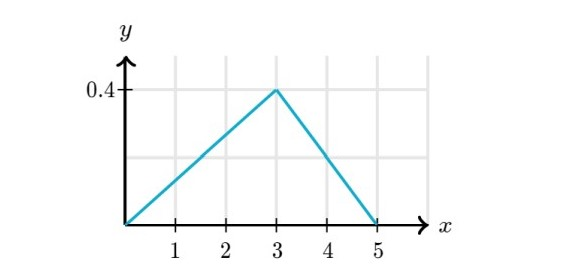
\includegraphics{DSgraph1.jpg}\\
\smallskip\\
\textbf{\underline{Answer}}\\
The probability $P(x>3)$ is the area below the line when $x>3$.\\
Triangle area is base times height divided by 2.\[
\frac{b\cdot h}{2}=\frac{2\cdot 0.4}{2}=0.4
\]
\[
\boxed{P(x>3)=0.4}
\]
 \newpage

\subsection{Question 6}
\textbf{\underline{Question}}\\
A company has 500 employees, and 60\% of them have children.
Suppose that we randomly select 4 of these employees.\\
What is the probability that exactly 3 of the 4 employees selected have children?
\smallskip\\
\textbf{\underline{Answer}}\\
60\% of the employees have children, which means $\frac{300}{500}$ employees.\\
Using the same method from Question 3, we write:\[
\binom{4}{1}\frac{200_{\textrm{ (no children)}}\cdot 300 \cdot 299 \cdot 298}{500 \cdot 499 \cdot 498 \cdot 497}=4\cdot 0.087=0.346
\]
\[
\boxed{P(\textrm{3 out of 4 have children})=0.346}
\]
\newpage

\subsection{Question 7}
\textbf{\underline{Question}}\\
Look at the next Graph. What is the expected value of X?\\
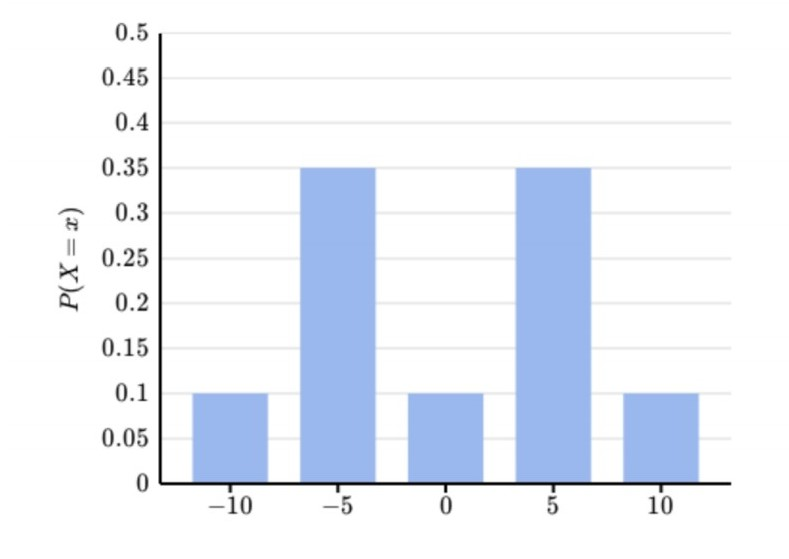
\includegraphics{DSgraph2.jpg}\\
\smallskip\\
\textbf{\underline{Answer}}\\
The expected value for discrete random variables is given by the formula:\[
E[X]=\Sigma^{k}_{i=1}x_i p_i
\]
so in our case:\[
-10\cdot 0.1+(-5)\cdot0.35+ 0\cdot 0.1 +5 \cdot 0.35 +10\cdot 0.1=0
\]
\[
\boxed{\textrm{Expected value of X is 0}}
\]









\end{document}